\documentclass[12pt,a4paper]{article}
\usepackage[utf8]{inputenc}
\usepackage[brazil]{babel}

% Melhorias na justificação do texto e
% pequenos ajustes em fontes e alinhamentos. 
\usepackage[T1]{fontenc}
\usepackage{microtype}

% Para fórmulas matemáticas
\usepackage{amsmath}

% Para listagens de programação ou 
% textos onde a formatação importa
\usepackage{listings}
\lstset{
	inputencoding=utf8,
    extendedchars=true,
	framextopmargin=2pt,
    framexbottommargin=2pt,    
    literate={á}{{\'a}}1
             {ã}{{\~a}}1
             {é}{{\'e}}1
             {í}{{\'i}}1
             {ç}{{\c{c}}}1
             {Ç}{{\c{C}}}1,
}
\renewcommand{\lstlistingname}{Listagem}% Listing -> Listagem
\renewcommand{\lstlistlistingname}{Lista de \lstlistingname s}% List of Listings -> Lista de Listagens

% Permite colocar figuras lado a lado ou
% fazer posicionamentos arbitrários
\usepackage[lofdepth,lotdepth]{subfig}

% Permite o uso da opção "frame" em "includegraphics"
% para fazer uma borda na imagem
\usepackage[export]{adjustbox}

% Para inserir gráficos e imagens
\usepackage{graphicx}
% Diretório padrão para figuras
\graphicspath{ {images/} }

\usepackage{hyperref}
\usepackage{abnt-alf}
\usepackage[top=3cm,bottom=2cm,left=3cm,right=2cm]{geometry}
\usepackage{indentfirst}
\usepackage{csquotes}

% Prefine que parágrafos (\paragraph) sejam colocados
% no índice. Isse permite usá-los livremente para
% formatação, caso contrário temos um erro se eles não
% estiverem dentro de uma subsubsection.
\setcounter{tocdepth}{3}

% Adiciona o comando \source para citar fontes abaixo
% de figuras. Muito útil!
\usepackage{caption}
\newcommand{\source}[1]{\vspace{-10pt} \caption*{Fonte: {#1}} }

% Facilita o copy 'n paste no PDF
% Remove ligaturas na cópia
%\input{glyphtounicode}
%\pdfgentounicode=1

% Texto colorido e afins. Bom para TODO notes
\usepackage{xargs}
\usepackage[pdftex,dvipsnames,table,xcdraw]{xcolor}
\usepackage[normalem]{ulem}
\useunder{\uline}{\ul}{}

% Símbolos diferentes para o texto, como setas →,
% símbolos de copyright e trademark, euro, etc.
% Não é muito útil, mas de vez em quando ajuda.
% Ao invés do comando do latex, dá pra usar o
% caractere em UTF-8.
\usepackage{textcomp}

% Todo notes.
% Muito útil para deixar anotações enquanto se está
% construindo o texto, depois dá para remover e onde
% quebrar são comentário que devem ser removidos.
\usepackage[colorinlistoftodos,prependcaption,textsize=tiny]{todonotes}
\newcommandx{\question}[2][1=]{\todo[linecolor=red,backgroundcolor=red!25,bordercolor=red,#1]{#2}}

\newcommandx{\change}[2][1=]{\todo[linecolor=blue,backgroundcolor=blue!25,bordercolor=blue,#1]{#2}}

\newcommandx{\info}[2][1=]{\todo[linecolor=OliveGreen,backgroundcolor=OliveGreen!25,bordercolor=OliveGreen,#1]{#2}}

\newcommandx{\draft}[2][1=]{\todo[linecolor=Plum,backgroundcolor=Plum!25,bordercolor=Plum,#1]{#2}}

\newcommandx{\thiswillnotshow}[2][1=]{\todo[disable,#1]{#2}}
\reversemarginpar
% END Todo notes.

\begin{document}

% CAPA
\pagestyle{empty}
\begin{center}
\large  \textbf{UNIVERSIDADE PRESBITERIANA MACKENZIE}
\large  \textbf{PROGRAMA DE PÓS-GRADUAÇÃO EM}\\
\large  \textbf{ENGENHARIA ELÉTRICA E COMPUTAÇÃO}\\
\vskip 2.0cm
\textbf{\large Ronie Miguel Uliana}\\
\vskip 4.0cm
\setlength{\baselineskip}{1.5\baselineskip}
\textbf{\MakeUppercase{\large Título a ser Definido}}\\
\vskip 4.5cm
\end{center}
\hfill{\vbox{\hsize=8.5cm\noindent\strut
Projeto de Pesquisa apresentado ao Programa\break
de Pós-Graduação em Engenharia Elétrica e\break
Computação da Universidade Presbiteriana\break
Mackenzie como parte dos requisitos para a\break
aprovação na disciplina de Metodologia do\break
Trabalho Científico.}\\
\strut}
\vskip 3.0cm
\textbf{\normalsize Orientador: Prof. Dr. Leandro Nunes de Castro}\\
\vskip 2.0cm
\begin{center}
São Paulo\\
2017\\
\end{center}

% RESUMO
\newpage
\thispagestyle{plain}
\pagenumbering{roman}
\begin{center}
\large
\textbf{RESUMO}
\end{center}
\renewcommand{\baselinestretch}{0.6666666}
A ser definido
\\[0.5cm]
\begin{flushleft}
{\bf Palavras-chave:} {\it apresentação, separada por vírgulas, de três a seis unitermos significativos para o trabalho.}
\end{flushleft}

% SUMÁRIO
\newpage
\thispagestyle{empty}
\tableofcontents

% DESENVOLVIMENTO
\newpage
\pagestyle{plain}
\pagenumbering{arabic}
\renewcommand{\baselinestretch}{1.5}
\normalsize

\listoftodos[Notas]

\section{INTRODUÇÃO}

Ao longo da vida profissional é comum para o indivíduo passar por diversas movimentações na carreira. Um estudante de engenharia pode iniciar como Trainee em uma empresa e progredir para Engenheiro, Supervisor de Obras e Diretor de Engenharia. Na área de computação é possível ver um Programador se tornar Analista-Programador, Coordenador de Desenvolvimento, Gerente de Projetos, chegando a Diretor de Operações. Esses são casos em que a movimentação de carreira segue um padrão mais tradicional de progressão, mas também há situações extremas de transições de carreira na qual um Analista-Programador resolve se tornar um Chef de Cozinha. Em qualquer um dos casos, as movimentações de carreira são sempre uma etapa de grande relevância profissional e que, ao mesmo tempo, podem causar estresse, insegurança e alguns desconfortos pelos novos desafios que surgirão.

Este projeto de pesquisa usa uma base de dados de mercado com 10 milhões de currículos e 23 milhões de experiências profissionais da empresa Vagas Tecnologia com o objetivo de fazer um estudo analítico sobre a movimentação de profissionais entre ocupações durante o curso de suas carreiras. O problema é modelado com uma estrutura em grafos e é analisado com conceitos e técnicas de Ciência da Redes.

Existem diversos trabalhos sobre movimentação profissional, principalmente sobre os fatores que motivam a mudança, como os expostos por~\citeonline{Ng2007-zp}~\todo{Ronie: tem mais uma série de papers, ler e mencionar (na introdução, talvez?)}. Porém, nenhum trabalho pôde ser encontrado analisando redes profissionais sob a ótica da Ciência de Redes, ponto onde esse trabalho tem sua maior contribuição.

A movimentação de profissionais é um ponto de interesse para pessoas, empresas e governo. Pessoas desejam saber onde podem chegar, empresas se interessam pela contratação e evolução de seus colaboradores e o setor público traça planos para suprir mão de obra onde ela é insuficiente ou criar oportunidades de trabalho onde ela é abundante. A pesquisa presente traz uma maior compreensão sobre como essa movimentação ocorre.

\section{REFERENCIAL TEÓRICO}

O objetivo deste capítulo é oferecer as bases conceituais necessárias ao estudo analítico das movimentações profissionais, como discutido anteriormente. Os principais conceitos necessários à pesquisa estão concentrados em Ciência de Redes. Cada um deles será apresentado como uma seção do capítulo, enfatizando apenas os aspectos necessários ao estudo analítico do projeto.

Para facilitar a compreensão do texto, abaixo são apresentadas definições para os termos encontrados no restante desse trabalho. Os significados são baseados livremente nos trabalhos de \citeonline{Wickham2014-qh} e \citeonline{Nunes2016}.

\begin{description}

	\item[Dados] são símbolos, textos ou números sem significado atribuído. Por exemplo, 2014, \enquote{verde} ou $\lambda$.

	\item[Informação] é um dado associado a um significado. Por exemplo, o câmbio entre Real e Dólar ser 3,10 no dia de hoje ou então que a última manutenção da estrada SP-250 foi em 2012.

	\item[Conhecimento] é uma informação que possui significado associado suficiente para a tomada de decisões. Por exemplo, saber que o dólar vai subir ou saber que as estradas para o interior estão em más condições.

	\item[Base de Dados] ou \textbf{Conjunto de Dados} é o conjunto de dados disponível.

	\item[Tabelas] são dados organizados em formato tabular onde as linhas são chamadas \textit{registros} ou \textit{objetos} e as colunas são chamadas \textit{atributos}, \textit{variáveis} ou \textit{campos}. Uma tabela representa um conjunto de registros de um mesmo tipo.

	\item[Objeto] descreve uma \enquote{unidade} sobre a qual temos informações. Também pode ser chamado \textbf{Registro} ou \textbf{Dado}.

	\item[Atributo] representa uma característica comum a todos os registros de um mesmo tipo. Um atributo dá significado a um valor e também pode ser chamado \textbf{Campo} ou \textbf{Variável}.

	\item[Valor] é o conteúdo de um atributo em um registro. Ele pode ser numérico, representando uma medição, grandeza ou ordem; um classe, representando um tipo ou classificação do registro; ou um texto, representando informação não estruturada.

\end{description}

\subsection{Considerações sobre Carreira}

A definir\ldots

\subsection{Ciência de Redes}

\todo[inline]{A definir\ldots Por enquanto, apenas algumas ideias soltas.}

Distância geodésica é um outro nome para o comprimento do caminho mais curto entre dois vértices, contado em número de arestas (ref).

\subsubsection{Métricas}

Densidade\ldots

Centralidades\ldots

Existem diversas medidas de centralidades em uma rede, as relevantes para o estudo e seu significado são descritas abaixo:\todo{Fazer uma introdução melhor}

\textbf{Betweness Centrality}

Explicar\ldots

(Útil para encontrar o vértice mais central. Aquele que está no meio das carreiras)

(Por que o peso das arestas, a grosso modo, representam a probabilidade de movimentação do profissional, a medida de centralidade que parece fazer mais sentido é a Betweeness Centrality baseado em Random Walk~\cite{Newman2005-la}).

\begin{figure}[ht]
  \centering
  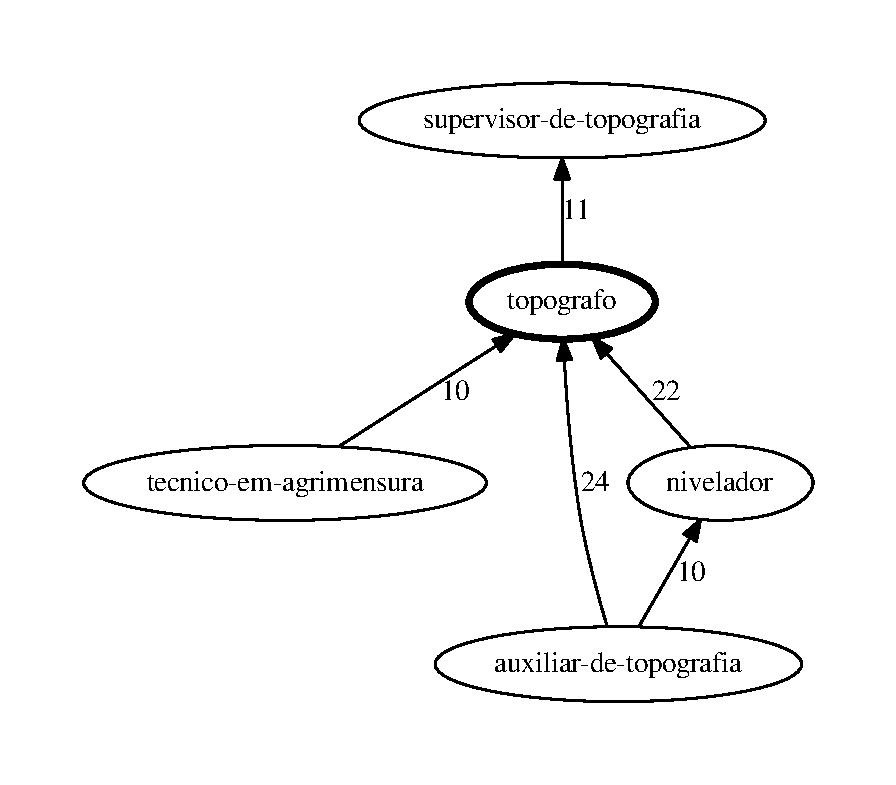
\includegraphics[scale=0.6]{cluster_25.pdf}
  \caption{Carreira de Topografia}
  \label{fig:carreira-topografia}
\end{figure}

\textbf{Nó de com maior número de caminhos até outro nós}

Verificar qual métrica é essa. Ela indica ocupações \enquote{de base}, ou seja, aquelas às quais é possível acessar o maior número de outras ocupações.

\textbf{Nó com maior número de caminhos de chegada}

Verificar qual métrica é essa. Ela indica ocupações que em que maior variedade de pessoas chega.


\subsubsection{Propriedades}

Scale free\ldots

Small world\ldots


\section{O MAPA DE CARREIRAS}

\subsection{Introdução}

O Mapa de Carreiras (MCar) traz o resumo da trajetória profissional de cerca de 10 milhões de pessoas e uma de suas manifestações pode ser vista no site \url{http://www.vagas.com.br/mapa-de-carreiras} (figura~\ref{fig:exemplo-grafo}). Internamente, essas informações estão armazenadas em um grafo e são periodicamente atualizadas. Nesse grafo, os vértices representam \textit{ocupações} e as arestas representam as \textit{movimentações} dos profissionais entre ocupações.

\begin{figure}[ht]
  \centering
  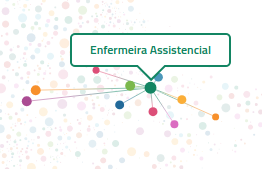
\includegraphics[scale=0.8, frame]{mapa-enfermeira-assistencial.png}
  \caption{Foco em uma ocupação}
  \source{Mapa de Carreiras}
  \label{fig:exemplo-grafo}
\end{figure}

No contexto do Mapa de Carreiras, uma \textit{ocupação} significa uma atividade profissional, remunerada ou não. A maior parte dessas ocupações são profissões remuneradas, tais como \enquote{Babá} ou \enquote{Arquiteto}, entretanto, algumas delas aparecem como atividade principal de uma pessoa, mas não são necessariamente uma profissão, tais como: \enquote{Mestrando}, \enquote{Enfermeiranda} ou \enquote{Voluntário}. Os vértices possuem diversos atributos que são resumos estatísticos daquela ocupação, tais como a distribuição salarial, a distribuição do tempo de permanência em uma ocupação, entre outras.

% ENTÃO UM VÉRTICE NA VERDADE SERÁ UM VETOR DE CARACTERÍSTICAS COM ESSAS INFORMAÇÕES. PRECISAMOS DEFINIR EXATAMENTE QUAIS CARACTERÍSTICAS COMPORÃO O VETOR DE CARACTERÍSTICAS DOS VÉRTICES. Ronie: Coloco isso dentro da Metodologia?

As arestas que conectam as ocupações representam \textit{movimentações} entre elas, ou seja, o fluxo de pessoas que exercia uma certa ocupação e passou a exercer outra. Acompanhar as arestas permite observar o movimento dos profissionais em suas carreiras. O peso das arestas é o número de profissionais que fizeram a trajetória de uma ocupação para outra. A figura~\ref{fig:exemplo-medico-do-trabalho} exibe as arestas a partir da ocupação \enquote{Médico do Trabalho} como exibidos pelo site do Mapa da Carreiras.

\begin{figure}[ht]
  \centering
  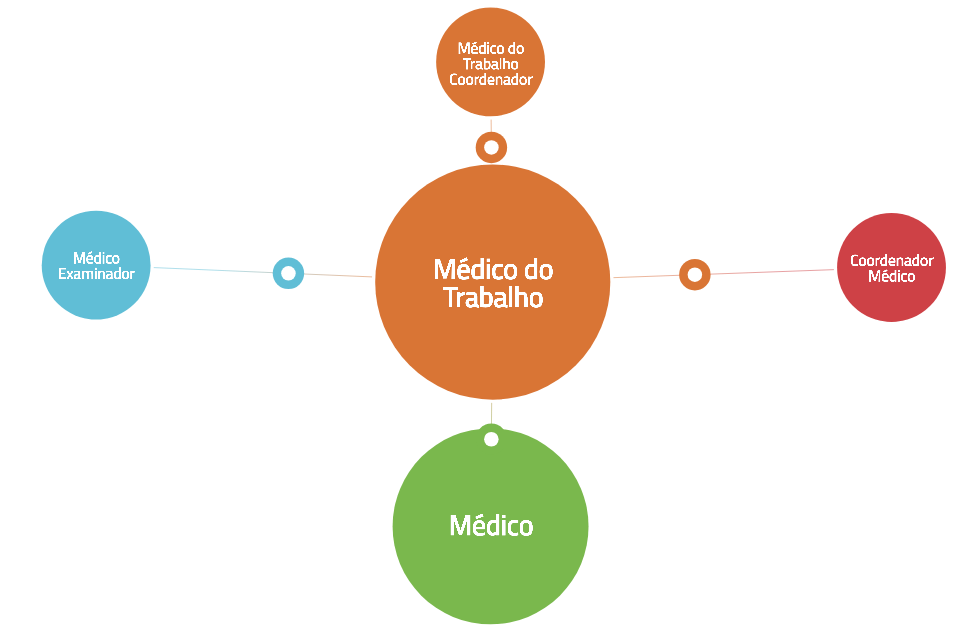
\includegraphics[scale=0.25]{mapa-medico-do-trabalho.png}
  \caption{Ocupações diretamente relacionadas a Médico do Trabalho}
  \source{Mapa de Carreiras}
  \label{fig:exemplo-medico-do-trabalho}
\end{figure}

É importante esclarecer que a visualização observada no site do Mapa da Carreiras foi construída para permitir uma navegação simplificada para o usuário (ref). Para essa pesquisa, os dados utilizados são os mesmos, mas em formatos mais adequados para essa pesquisa. Por exemplo, o equivalente da figura~\ref{fig:exemplo-medico-do-trabalho} utilizada para análise exploratória pode ser vista na figura~\ref{fig:grafo-medico-do-trabalho}. Nela, é possível observar ocupações que não estão diretamente relacionadas a \enquote{Médico do Trabalho}, mas que estão no mesmo agrupamento, como \enquote{Médico Plantonista}.

\begin{figure}[ht]
  \centering
  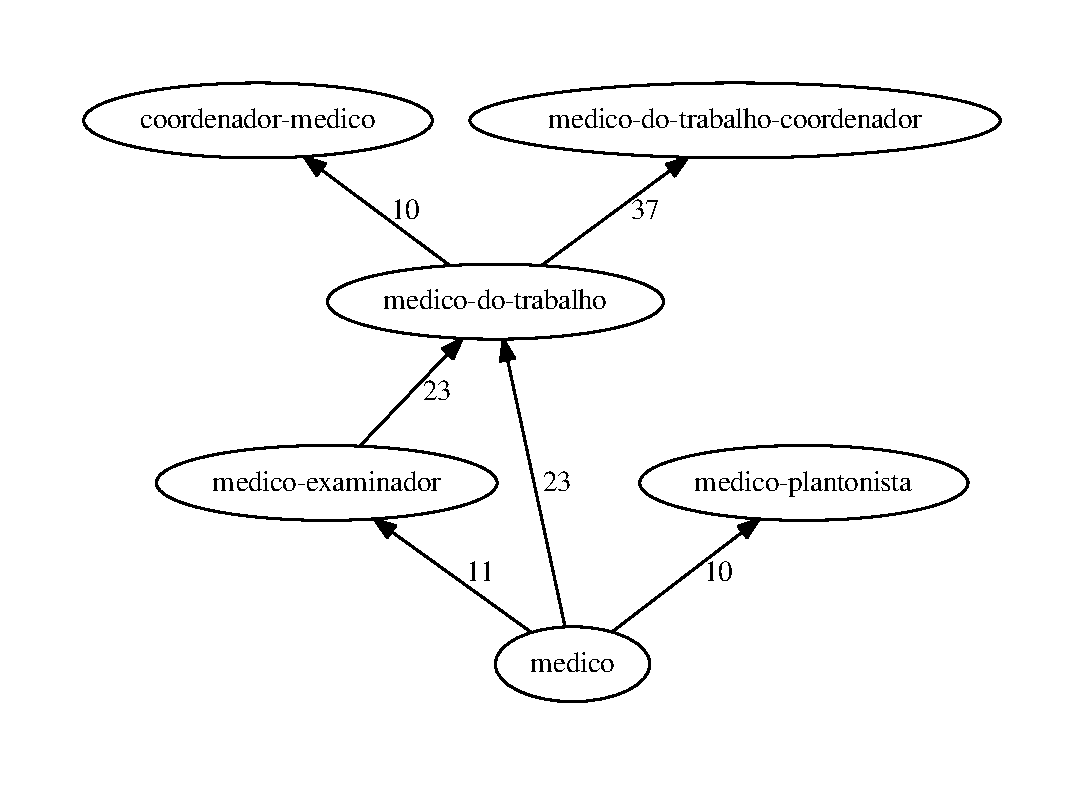
\includegraphics[scale=0.6]{cluster_24.pdf}
  \caption{Grafo ao redor de Médico do Trabalho}
  \source{Elaboração do autor}
  \label{fig:grafo-medico-do-trabalho}
\end{figure}

O grafo do MCar é direcionado e, portanto, o fluxo de profissionais entre ocupações possui uma direção específica, mas é comum que existam movimentações em ambos os sentidos entre duas ocupações. Esse movimento é representado por duas arestas diferentes, mesmo que no site ela seja representada por uma única aresta. Em outras palavras, o MCar é um grafo direcionado com ciclos, porém os vértices não são autorreferentes.

Por conta dos ciclos, não é possível criar uma ordenação topológica que represente uma clara progressão de carreira para o grafo como um todo. Entretanto, é possível extrair grupos de ocupações que possuem movimentações mais frequentes entre si. Esses agrupamentos são comumente acíclicos, o que possibilita traçar essa progressão entre as ocupações que o compõem. Nos experimentos do Capítulo XX é possível observar que essa característica é mais frequentemente observada em grupos formados por ocupações que requerem maior qualificação técnica, como \enquote{Comércio Exterior} ou \enquote{Médico do Trabalho}, como visto na figura~\ref{fig:grafo-medico-do-trabalho}. Já nas ocupações ditas \enquote{operacionais}, o fluxo de movimentação entre ocupações acentua a característica cíclica do grafo. Particularmente, é possível observar um forte ciclo entre as ocupações \enquote{Recepcionista}, \enquote{Vendedor} e \enquote{Auxiliar Administrativo}, como mostrado pela figura~\ref{fig:grafo-ciclo-operacional}.

\begin{figure}[ht]
  \centering
  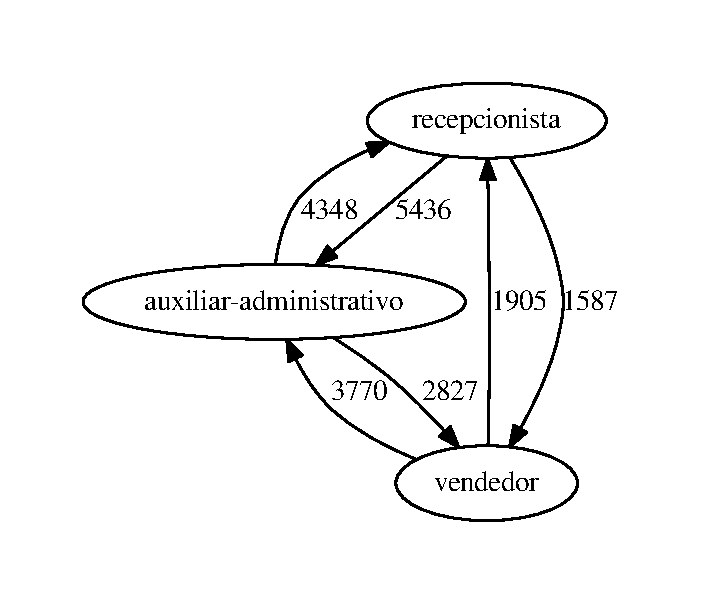
\includegraphics[scale=0.8]{ciclo-operacional.pdf}
  \caption{Ciclo entre Ocupações}
  \source{Elaboração do autor}
  \label{fig:grafo-ciclo-operacional}
\end{figure}

Para a construção dos vértices, os textos presentes nos títulos dos históricos profissionais dos currículos foram \enquote{normalizados}. Nesse contexto, \enquote{normalização} significa transformar os títulos com o mesmo significado na mesma representação textual. Por exemplo, a mesma ocupação pode ter sido registrada por pessoas diferentes como \enquote{Moto Boy}, \enquote{moto boy}, \enquote{Motoboy}, \enquote{Moto Girl} entre outras variações. O que chamamos de \enquote{normalização} é o trabalho de transformar essas diferentes grafias em uma única classe que possa ser usada para identificação da ocupação. No caso, todas as anteriores são normalizadas para \enquote{motoboy}. Esse trabalho também inclui a correção ortográfica e a remoção de abreviação das ocupações.

Após a normalização são criados pares de ocupações cronologicamente ordenados. Isso significa que o término de uma ocupação precisa coincidir com o início da seguinte. Uma margem de dois meses de tolerância na sobreposição corrige pequenas imprecisões na anotação dos históricos profissionais. Currículos com apenas uma ocupação são descartados, bem como ocupações que se sobreponham cronologicamente ou que estejam separadas por um intervalo de tempo maior que um ano.

Os pares de ocupações são unificados produzindo as arestas e os vértices, e as arestas menos relevantes do grafo são podadas. Arestas com menos de dez movimentações são removidas do grafo e vértices sem conexão depois desse processo são removidos. Esse critério de poda foi definido empiricamente através de análise por amostragem. Números muito maiores removem vértices de ocupações mais especializadas como \enquote{Comandante} ou \enquote{Engenheiro de Minas}, enquanto números muito menores acrescentavam vértices espúrios causados por erros de grafia que a fase de correção ortográfica foi incapaz de detectar.

Um dos efeitos indesejados desse processo é que algumas ocupações legítimas são removidas do grafo. É o caso de ocupações muito recentes, muito especializadas, ou que ainda não possuem uma concordância da nomenclatura entre os profissionais da área. Como exemplo podemos citar \enquote{Especialista em Experiência do Usuário}, uma profissão recente, que também é chamada \enquote{Analista de UX} ou apenas \enquote{UX}.

Duas outras limitações no grafo ocorrem por conta da experiência profissional ser um campo de texto livre, ou seja, o usuário digita livremente sua ocupação sem estar restrito a uma lista de opções. A primeira se refere a ocupações que foram digitadas para representar uma ocupação dupla, como \enquote{Caixa e Balconista} ou \enquote{Atendente/Estoquista}. A segunda ocorre por ambiguidade no nome da ocupação, como \enquote{Coordenador de Projetos}, que ocorre na carreira de Desenvolvimento de Software e na de Engenharia Civil.

Por outro lado, o campo de texto livre permite a captura de ocupações que pouco provavelmente apareceriam em uma lista curada, como \enquote{IRLA} (Instalador Reparador de Linhas Aéreas) ou \enquote{Rigger} (pessoa no solo que orienta o posicionamento de carga para o operador de guindaste).

Ao final do processo o grafo possui cerca de 8.348 ocupações distintas e 14.031 arestas. Esses números flutuam dependendo das atualizações dos currículos em que são baseados e no crescimento natural do banco de dados. Os dados presentes nesse trabalho refletem a base atualizada em Fevereiro de 2017.


\subsection{O Processo de Construção do Mapa de Carreiras} \label{sec:construcao}

O Mapa de Carreiras é construído a partir dos currículos de um banco relacional condensando seus dados para formar um grafo de movimentação de pessoas entre as ocupações.

As seções a seguir descrevem os passos envolvidos na montagem do grafo.

\subsubsection{Os Dados}

Os dados fonte para essa pesquisa são currículos anonimizados de usuários do site de carreiras VAGAS.com.br. Esses currículos são armazenados em um banco de dados \textit{Microsoft SQL Server}. No total há cerca de 10 milhões de currículos~\todo{Colocar número exato} armazenados entre 1999 e 2016, mas para esse trabalho apenas os currículos atualizados entre 2011 e 2016 são utilizados~\todo{Colocar número exato}.

% FALE AGORA DOS CVS DA ÁREA DE TECNOLOGIA. QUANTOS SÃO? QUANTAS E QUAIS SÃO AS CARREIRAS (A LISTAGEM DAS CARREIRAS PODE VIR COMO UM APÊNDICE)
% Ronie: Focamos ainda na área de tecnologia? Acredito que poderíamos focá-la nos exemplos de carreiras maiores (como análise das redes livre de escala e mundo pequeno) que não são boas com carreiras muito pequenas como as que usei acima para exemplificar alguns grafos. Que acha?

Para as análises a serem explicadas nesse capítulo, os dados são primeiramente extraídos para arquivos textos e só então processados. Existem dois formatos usados nesse trabalho. O primeiro formato é descrito por \citeonline{Van_Dongen2008-kx} como \enquote{formato ABC}. Cada linha representa uma aresta, e cada aresta possui três campos separados por um ou mais espaços. Em um grafo direcionado, o primeiro campo é a aresta de partida, o segundo é a aresta de chegada e o campo final representa o peso da aresta. No caso do MCar, o peso representa o número de pessoas que se movimentou de uma ocupação à outra. Esse formato é usado na separação de carreiras através da \textit{clusterização} do grafo usando o \textit{Markov Clustering Algorithm} (MCL)~\cite{Van_Dongen2000-qm} e na montagem de visualizações exploratórias usando o programa \enquote{Graphviz}~\cite{Gansner2000-oo}.

\noindent\begin{minipage}{\linewidth}
\begin{lstlisting}[frame=single,caption=Arquivo em Formato ABC,label=lst:formato-abc,captionpos=b]
medico-examinador medico-do-trabalho 23
medico-do-trabalho coordenador-medico 10
medico-do-trabalho medico-do-trabalho-coordenador 37
medico medico-plantonista 10
medico medico-examinador 11
medico medico-do-trabalho 23
\end{lstlisting}
\end{minipage}

O segundo formato é uma lista de registros onde cada um ocupa uma única linha. Cada registro é codificado como uma \textit{array} de atributos no formato JSON (\textit{Javascript Object Notation}). Esse formato é usado em várias etapas da montagem do MCar e seu conteúdo varia de etapa para etapa. Os campos relevantes são descritos nas seções adequadas a seguir.

\subsubsection{O Processamento da Informação}

O volume de dados e a variedade de análises desse trabalho impõe algumas restrições de ordem prática que precisam ser contornadas. O volume de dados é grande o suficiente para exceder a memória de um computador convencional, algumas das ferramentas utilizadas não se comunicam com outras exceto através de arquivos texto e o tempo para processamento facilmente excede alguns dias se os processadores não forem adequadamente utilizados.

Essas restrições e a necessidade de atualizar continuamente os dados do MCar levaram a implementação de um sistema que executasse todos os passos para sua montagem de maneira automática.

A informação é processada em uma série de etapas consecutivas usando um padrão arquitetural conhecido como \textit{Dataflow}~\cite{Carkci2014-jk, Hohpe2003-nj}, especificamente o modelo conhecido como \textit{Pipes and Filters} ou \textit{Pipeline}. Nesse padrão, os dados fluem continuamente de um processo para o outro, sendo transformados e filtrados conforme o processo avança. 

Em uma estrutura de \textit{pipeline}, com exceção de alguns componentes especiais, cada processo possui apenas uma interface de entrada e uma interface de saída. Desde que mantenha a mesma interface, um processo pode ser substituído por outro, ou por um conjunto deles, sem afetar outras partes do sistema.

Essa arquitetura foi implementada em máquinas \textit{Linux} utilizando \textit{pipes} e \textit{sockets} para comunicação interprocessos. Um \textit{pipe} no \textit{Linux} é uma implementação de FIFO em memória RAM. A interface para \textit{push} na fila é idêntica a gravação de uma linha de texto em um arquivo. Do outro lado um outro processo lê a fila com a mesma interface de leitura de um arquivo linha a linha. Por usar interfaces compatíveis que leituras e gravações em arquivo, qualquer programa capaz de executar essas operações pode ser usado como parte do \textit{pipeline}. Isso resolve o problema do uso de ferramentas díspares, desde que sejam capazes de gravar e ler em arquivos texto, são capazes de se integrar ao processo como um todo.

Enquanto \textit{pipes} permitem a comunicação interprocessos na mesma máquina, \textit{sockets} podem ser usados para comunicação entre computadores através de uma interface padronizada. Ao invés dos \textit{sockets} nativos do \textit{Linux}, optou-se pelo \textit{ZeroMQ} que é uma implementação mais robusta, criada para transmitir dados usando diversos modelos de distribuição~\cite{Hintjens2013-tz}.

O \textit{ZeroMQ} possui interfaces para diversas linguagens de programação, mas para preservar a interface entre processos foram criados componentes que traduzem a entrada em \textit{pipes} para \textit{sockets ZeroMQ} e vice-versa. Em termos práticos, a comunicação entre processos pode ser feita entre processos da mesma máquina ou entre diferentes computadores de maneira transparente.

A maior parte dos processos foi implementada usando a linguagem Ruby, mas alguns processos foram implementados usando Python ou programas específicos, como o MCL para \textit{clusterização} e o Graphviz para posicionamento do grafo em um plano bidimensional.

A montagem do grafo é mostrada na figura~\ref{fig:montagem-do-grafo}.

\begin{figure}[ht]
  \centering
  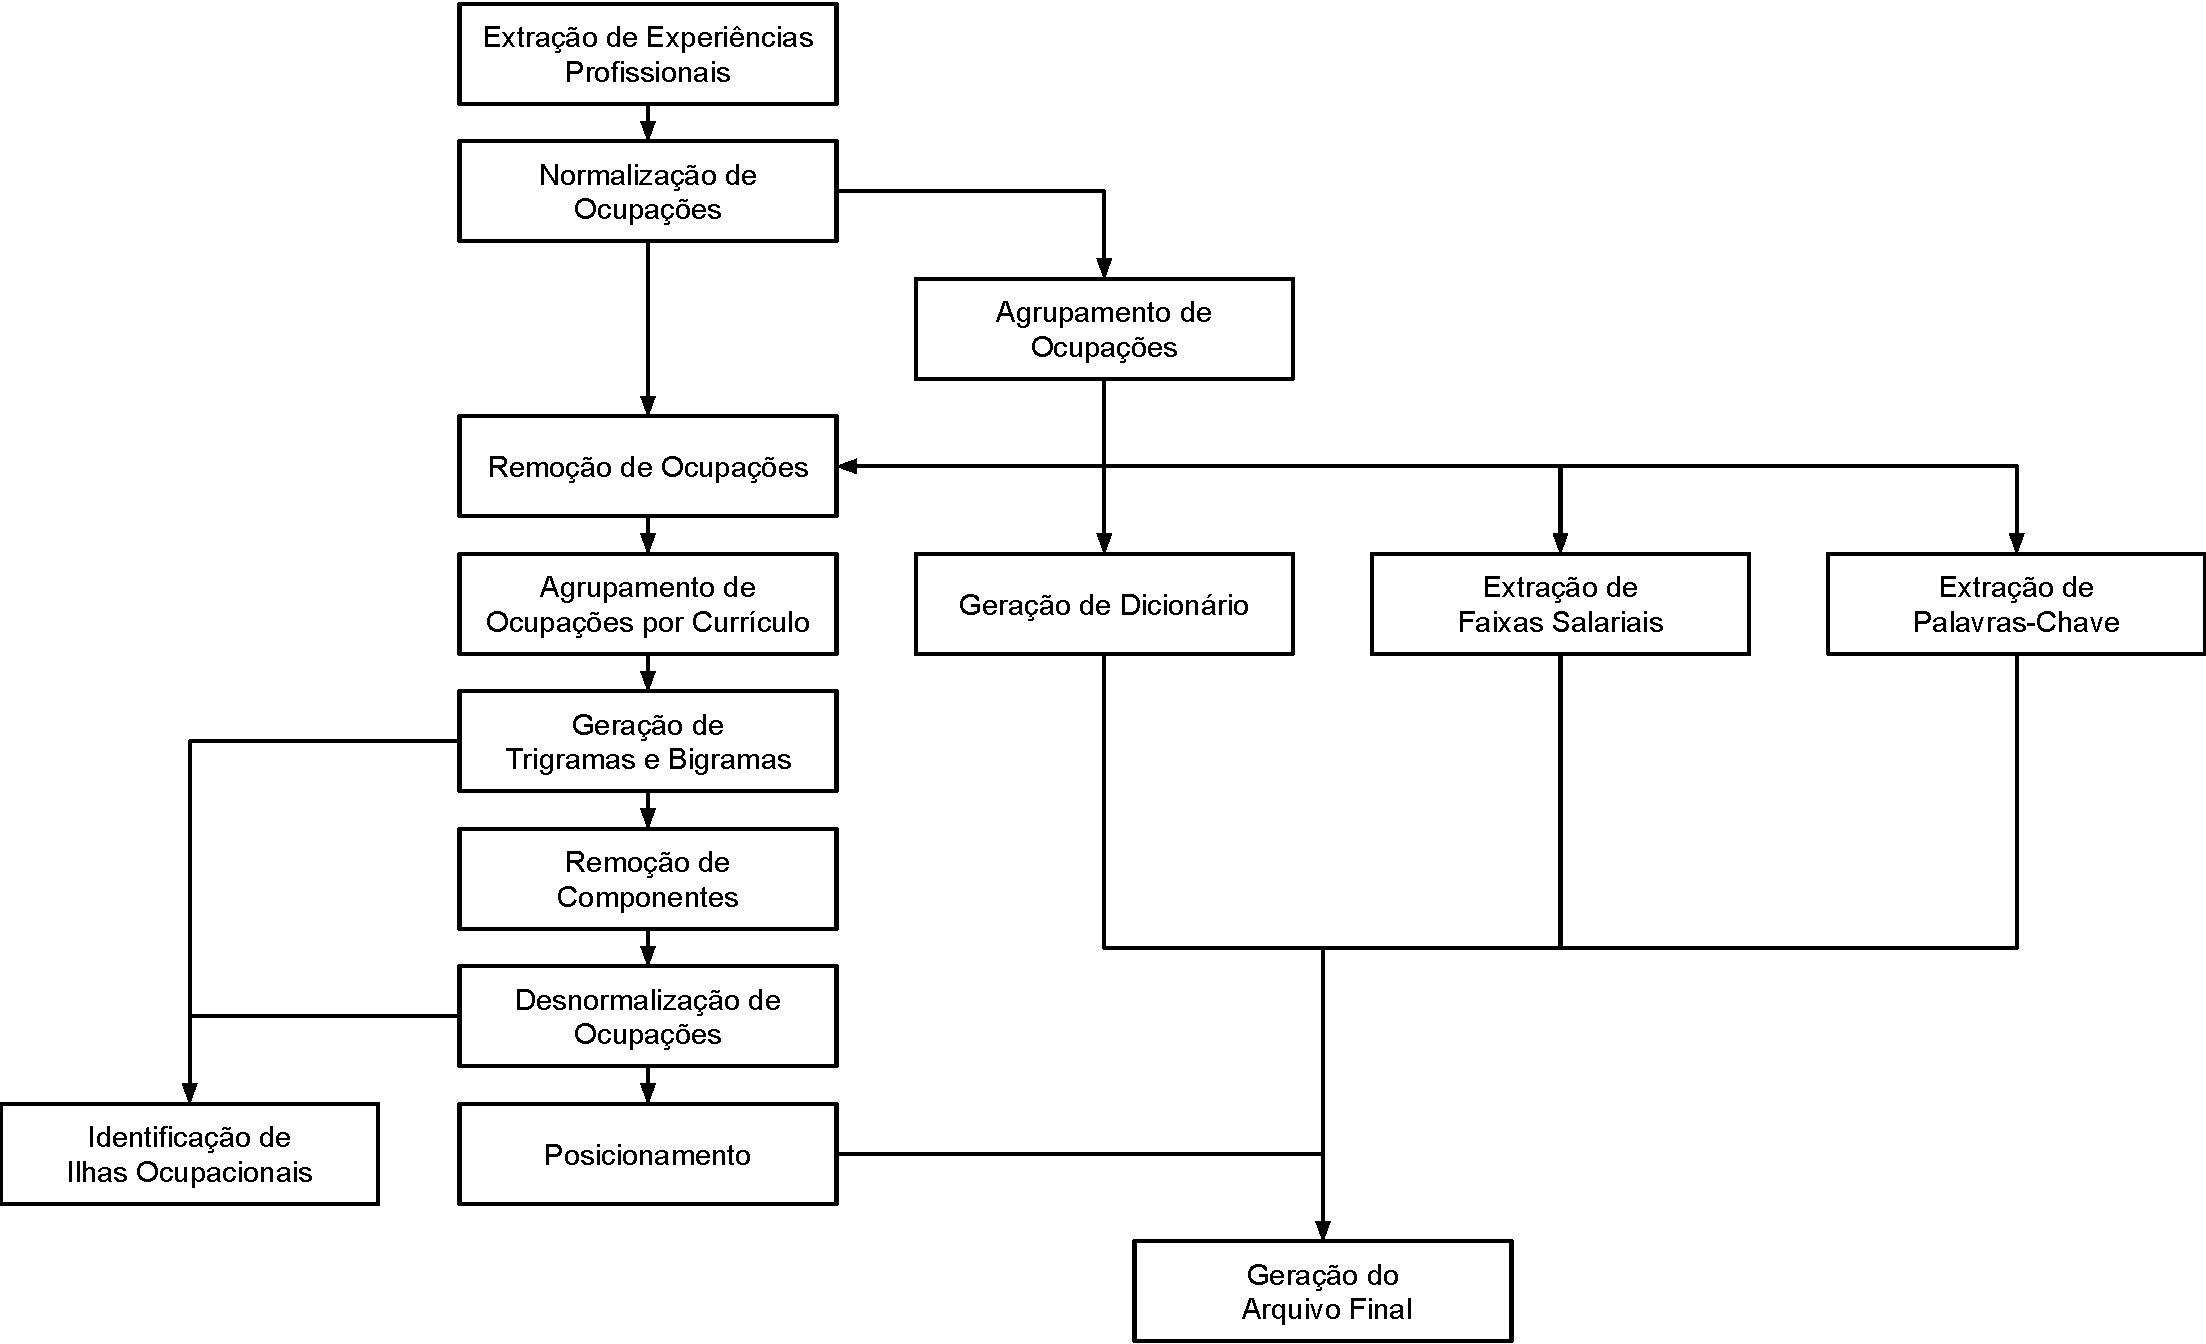
\includegraphics[scale=0.4]{pipeline1.pdf}
  \caption{Montagem do Grafo}
  \label{fig:montagem-do-grafo}
\end{figure}

\subsubsection{Extração do Experiências Profissionais} \label{sec:extracao-experiencia}

O primeiro processo do \textit{pipeline} extrai os registros do bancos de dados relacional e os grava em arquivos texto. O processo não extrai currículos, mas sim experiências profissionais. Cada registro representa uma única experiência.

Os dados extraídos são:

\begin{description}

  \item[Identificador do Currículo] é um número único para cada currículo dentro do banco de dados. Ele é usado posteriormente para agrupar as experiências profissionais por pessoa.

  \item[Nome da Ocupação] é o texto digitado livremente pelo usuário no campo nomeado \enquote{Cargo} no currículo. Esse texto dá origem aos nomes das ocupações usadas no Mapa de Carreiras.

  \item[Data de Início] e \textbf{Data de Término} marcam quando o profissional iniciou naquela ocupação e até quando a exerceu. Se é a ocupação atual, não existe uma data de término. Esses campos são usados para determinar a sequência de experiências profissionais que formarão as arestas do grafo.

  \item[Texto Descritivo] é o texto digitado livremente pelo usuário no campo com o nome \enquote{Descrição} no currículo. Esse campo é usado para criar uma nuvem de palavras-chave sobre a ocupação.

\end{description}

\subsubsection{Normalização de Ocupações} \label{sec:normalizacao}

Nessa etapa, o nome da ocupação é normalizado para uma classe de maneira que todas as grafias significando a mesmo ocupação sejam transformadas em uma mesma classe. Nessa pesquisa a classe é chamada \enquote{classe equivalente} ou \enquote{ocupação normalizada}.

Para transformar o texto digitado em uma ocupação normalizada os erros de digitação são corrigidos, pontuações são removidas, abreviaturas frequentes são expandidas, o texto é colocado em minúsculas, é feita a singularização das palavras que compõem a ocupação e os nomes são masculinizados (\enquote{secretária} se transforma em \enquote{secretário}, por exemplo).

Ocupações com múltiplas palavras também são ordenadas alfabeticamente. Dessa forma, ocupações como \enquote{Auxiliar Financeiro-Administrativo} e \enquote{Auxiliar Administrativo-Financeiro} resultam na classe \enquote{administrativo auxiliar financeiro}.

As classes resultantes lembram vagamente o termo original, como no exemplo acima. No processo descrito na seção~\ref{sec:criar-dicionario}, é criado um dicionário entre a classe equivalente e um nome que tenha significado para o usuário.

\subsubsection{Remoção de Ocupações Incorretas} \label{sec:remocao-ocupacoes-incorretas}

Mesmo após a remoção de casos únicos, alguns nomes presentes nesse campo não podem ser realmente considerados ocupações. São erros comuns que a etapa de normalização não é capaz de corrigir ou representam um entendimento errôneo por parte do usuário.

Casos emblemáticos são os textos \enquote{sim}, \enquote{não} ou \enquote{o mesmo} encontrados no campo destinado ao nome da ocupação. A remoção desses casos precisou ser feita manualmente, especialistas da empresa revisaram a lista de ocupações e criaram um dicionário com os erros mais comuns utilizado nessa etapa do processo. Esse dicionário foi aprimorado com sugestões dos usuários após a publicação do MCar.

\subsubsection{Agrupamento de Ocupações por Currículo}

As ocupações são agrupadas por currículo, formando uma sequência cronológica das experiências de um profissional.

Até essa etapa, há uma experiência profissional por registro, após ela, cada registro contém uma sequência de experiências profissionais do mesmo indivíduo, ordenadas cronologicamente.

% Inserir um diagrama com os campos. Ronie 2017-04-30

\subsubsection{Remoção de Experiências sem Conexão ou Sobrepostas}

Como o objetivo final é criar um grafo que sumarize o \textit{movimento} de pessoas entre ocupações, as experiências profissionais que não se conectam cronologicamente com nenhuma outra são removidas.

Considerar-se desconexa quaisquer experiências em sequência cujo início da posterior esteja a mais do dois meses de distância do fim da anterior.

% Inserir um gráfico explicativo. Ronie 2017-02-30

Na mesma etapa, removem-se experiências profissionais que se sobreponham. Uma vez sobrepostas, não é possível afirmar que uma é sequência natural da outra ou que sequer tenham relação entre si. É comum encontrar no banco de dados carreiras paralelas em que gestores também são professores ou técnicos que também sejam voluntários. Da mesma maneira que experiências desconexas, as que se sobrepõem por mais de dois meses são removidas.

\subsubsection{Remoção de Currículos por Experiência}

Após o processo anterior, são removidos os registros que possuam apenas uma ou nenhuma experiência profissional.

\subsubsection{Geração de Pares de Experiência}

As experiências profissionais de cada currículo são pareadas por ordem cronológica. Por exemplo, um currículo que tenha a seguinte sequência de ocupações \enquote{Faxineiro \textrightarrow~Copeiro \textrightarrow~Chapeiro}, produz os pares \enquote{Faxineiro \textrightarrow~Copeiro} e \enquote{Copeiro \textrightarrow~Chapeiro}.

Antes desse processo, cada registro é uma sequência de experiências profissionais. O processo explode cada registro em múltiplos registros, cada um representando um par de experiências profissionais de um único indivíduo.

\subsubsection{Agrupamento de Pares de Ocupações}

Pares iguais de ocupações são agrupados e contados, gerando um \textit{multiset}, ou seja, um conjunto com o número repetições de cada elemento. O número de repetições em um par representa o número de pessoas que se movimentaram de uma ocupação para outra.

As etapas posteriores podam o grafo em suas arestas menos relevantes e transformam sua representação textual para que possa ser lido por outros programas.

\subsubsection{Remoção de Pares Pouco Frequentes} \label{sec:grafo-final}

A maior parte dos pares de ocupações ocorrem pouquíssimas vezes. Em um conjunto com XX pares, cerca de XX ocorrem apenas uma vez. Esse pequeno número de repetições é causado tanto por trajetórias incomuns quanto por erros de digitação que as etapas anteriores não foram capazes de eliminar. Por vezes, são apenas ocupações similares a outras, mas onde os usuários escrevem de maneira pouco convencional. Com alguma frequência, os pares realmente representam trajetórias em carreiras extremamente específicas.

Para encontrar um número de corte foi feita uma avaliação manual por amostragem. Amostras com algumas centenas de pares com números de corte entre 1 e 30 foram analisadas por especialistas da empresa junto com o pesquisador. O objetivo foi encontrar um número que não fosse conservador demais, removendo trajetórias válidas, nem liberal demais, permitindo trajetórias com erro.

Após o processo de análise, chegou-se a um número próximo a 10 repetições. Pares de ocupações com menos de 10 repetições são removidos.

A partir desse ponto, os dados para a montagem do grafo estão prontos em formato texto.

\subsubsection{Posicionamento dos Vértices do Grafo}

Para que o grafo possa ser exibido bidimensionalmente, é preciso que seus vértices sejam posicionados de modo a evitar a sobreposição e que os vértices relacionados por arestas de maior peso estejam mais próximas.

O algoritmo de \textit{Force-Directed} (ref) é usado para posicioná-los corretamente. Esse algoritmo é aplicado nesse passo utilizando o programa Graphviz.

A saída do Graphviz é um arquivo texto com a posição X e Y do vértice em um plano cartesiano.

\subsubsection{Descoberta de Proto-Carreiras}

% Me parece que "proto-carreiras" não é um nome lá muito bom, mas foi o que consegui por enquanto =/ Ronie 2017-04-29
% Aqui também tem uma dose não saudável de especulação baseado no tempo que fiquei olhando para esse grafo. Pode ser o caso de colocar números em tudo (gosto disso), ou eliminar boa parte do texto. Ronie 2017-04-30

O grafo gerado no passo~\ref{sec:grafo-final} é usado nesse processo para gerar agrupamentos.

Entre duas ocupações, o maior fluxo de movimentações indica uma certa preferência por uma das duas. Por exemplo, se o número de movimentações entre \enquote{Analista da Sistemas \textrightarrow~Coordenador de Projeto} for maior que o reverso \enquote{Coordenador de Projeto \textrightarrow~Analista da Sistemas}, considera-se que \enquote{Coordenador de Projeto} é uma ocupação que sucede \enquote{Analista de Sistemas}. Algumas vezes, o fluxo entre as ocupações é tão similar que não é possível dizer que há uma ordem de sucessão, como no caso apresentado no ciclo de ocupações operacionais na figura~\ref{fig:grafo-ciclo-operacional}; em outros, o sentido contrário possui um fluxo várias vezes menor ou não há fluxo contrário, como o caso do grafo sobre \enquote{Médico do Trabalho} na figura~\ref{fig:grafo-medico-do-trabalho}.

\todo[inline]{Ronie: estou pensando que a seção abaixo pode ser movida para \enquote{conclusões} ou mais para frente, que acha?}

Quando o fluxo de pessoas de uma ocupação para outra é relevante, é possível notar que essa ordem de preferência vai normalmente de ocupações mais operacionais e com salários mais baixo para ocupações mais gerenciais e com salários mais altos. O que coincide com a senso comum de progressão de carreira.

A grosso modo, o agrupamento e o fluxo de migração das ocupações revela o que se pode considerar um \enquote{protótipo de carreira}. Ou seja, um esboço onde um indivíduo em uma ocupação dentro desse grupo tem uma probabilidade maior de se manter nele e de se movimentar para ocupações no topo do grupo.

Existe, no entanto, um grupo que não obedece às características descritas acima. Ao se tentar ordená-lo topologicamente, não há uma ordem de preferência clara entre as ocupações, o que indica que não há uma noção sucessão como em outros grupos como exemplificado anteriormente na figura~\ref{fig:grafo-ciclo-operacional}. Ele também possui algumas ocupações que conectam uma grande quantidade de outras ocupações, como \enquote{Auxiliar Administrativo} que possui movimentações com XX ocupações, cerca de XX\% das ocupações do MCar.

Ao analisar o grupo, nota-se que a escolaridade mais frequente nessas ocupações é a de \enquote{segundo grau completo}, significando que essas ocupações não necessitam de treinamento especializado para serem desempenhadas, o que é um indício que esse grupo reflete a própria definição de \enquote{operacional}.

Algumas outras ocupações também possuem \enquote{segundo grau completo} como escolaridade mais frequente, mas se comportam como os grupos com uma direção clara de preferência entre as ocupações. Uma análise manual da descrição das suas ocupações e das palavras-chave relacionadas sugere que essas são ocupações \enquote{técnicas}. Ou seja, uma ocupação que requer um treinamento não-trivial, mas não tão exigente quanto uma graduação. Como exemplo, é possível observar a carreira de cozinheiro na figura~\ref{fig:exemplo-grafo-cozinheiro}.

\begin{figure}[htb]
  \centering
  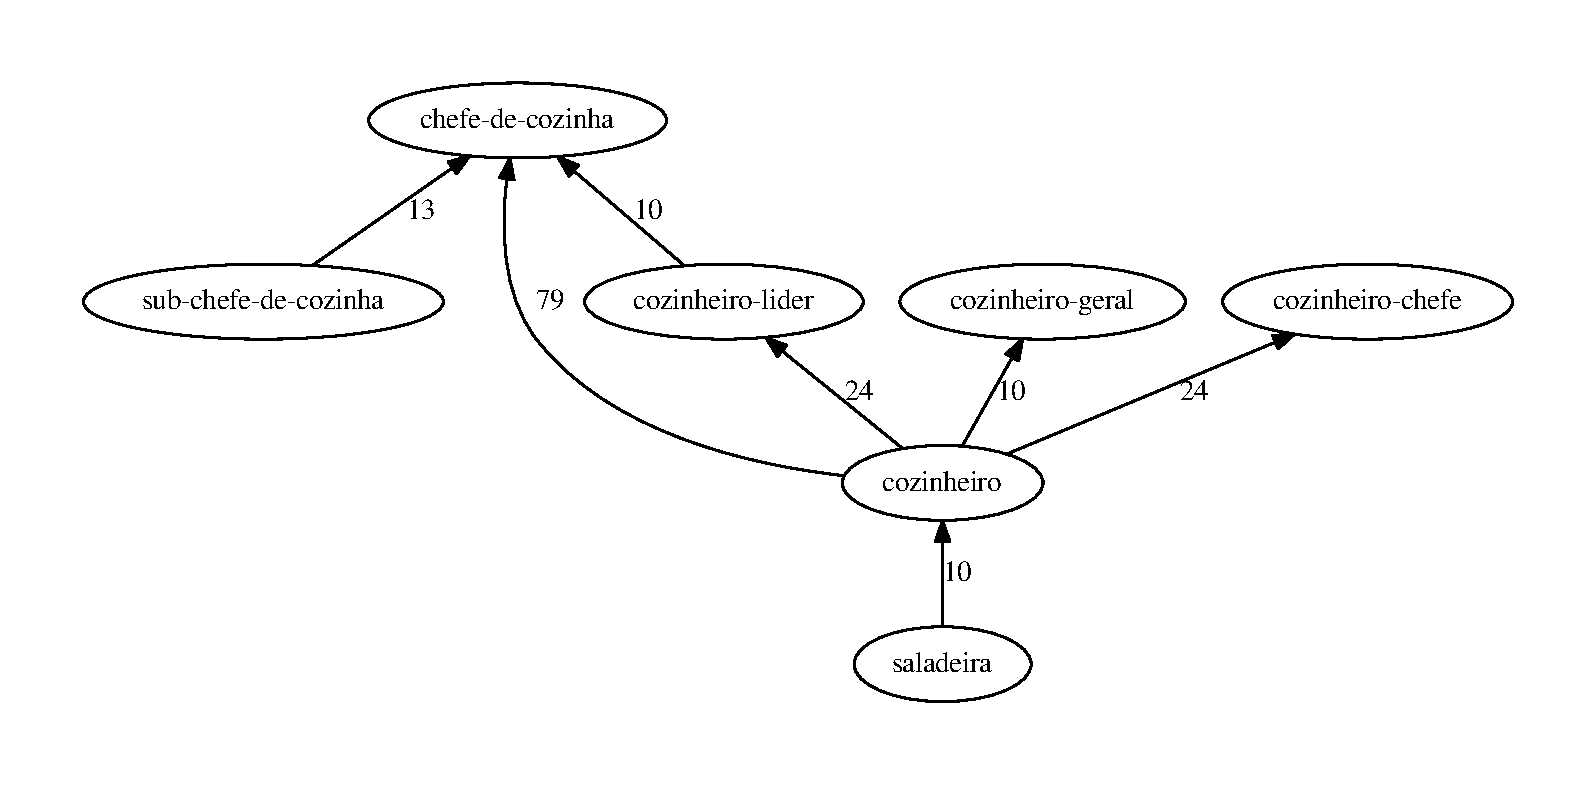
\includegraphics[scale=0.6]{subcluster_01_11.pdf}
  \caption{Carreira Técnica de Cozinheiro}
  \label{fig:exemplo-grafo-cozinheiro}
\end{figure}

\subsubsection{Agrupamento de Ocupações}

Esse processo agrupa os dados gerados pelo processo descrito na seção\ref{sec:remocao-ocupacoes-incorretas} por ocupação. Cada ocupação normalizada agora possui uma lista com suas grafias originais, uma lista com as descrições daquela experiência profissional escrita por cada indivíduo, bem como a quantidade de ocupações agrupadas.

\subsubsection{Remoção de Ocupações com Pouca Frequência}

Mesmo com o processo de correção e normalização, algumas experiências profissionais são escritas de maneira única. Isso pode significar um erro, uma ocupação singular ou o uso de termos pouco convencionais. Como o objetivo da montagem do grafo é extrair as carreiras mais frequentes, os casos únicos podem ser seguramente removidos sem a necessidade de determinar sua causa.

\subsubsection{Criação de Dicionário para Exibição} \label{sec:criar-dicionario}

Os textos resultantes do processo de normalização descrito na seção~\ref{sec:normalizacao} não são adequadas para exibição. Esse processo contabiliza o número de grafia exatamente idênticas para cada ocupação normalizada e assume como \enquote{nome de exibição} a grafia mais frequente.

A limitação desse processo é que algumas ocupações são descritas no masculino ou no feminino dependendo do número de profissionais do gênero exercendo esse ocupação. Por exemplo: uma das ocupações de Direito é descrita como \enquote{Advogado} (no masculino) pois existem um pouco mais profissionais do gênero masculino exercendo a profissão, por outro lado, uma outra ocupação correlacionada é descrita como \enquote{Advogada Coordenadora} pelo motivo contrário.

Apesar da regra da língua portuguesa do uso do masculino quando há um grupo de gênero misto (ref), optou-se por não se modificar o gênero artificialmente, preservando a grafia da predominância do gênero na ocupação.

\subsubsection{Extração de Palavras-Chave}

As palavras-chave são extraídas a partir das descrições digitadas pelos usuários no campo \enquote{Experiência Profissional} dos currículos.

O processo descrito abaixo tenta criar expressões significativas, ou seja, pequenas frases, que ajudem a descrever o cargo ao invés de apenas indicar as palavras mais comuns.

Um fato notável é que não é possível utilizar \textit{stemming} ou de correção ortográfica nesse processo, pois existe uma grande quantidade de jargões e siglas específicos nas descrições.

Para formar expressões, são gerados unigramas, bigramas e trigramas para as descrições de cada experiência profissional. A seguir, elas são ordenadas por TF-IDF e as palavras que aparecem repetidas em um n-grama de menor TF-IDF são removidas. Por exemplo, se a palavra \enquote{fiscal} aparece com maior TF-IDF que o bigrama \enquote{nota fiscal}, a palavra \enquote{fiscal} é removida da lista.

% Na prática, o resultado é muito bom, mas o algoritmo foi baseado no meu nariz =/ Então, talvez eu devesse refazer o processo com uma técnica de sumarização melhor.

\subsubsection{Gravação do Arquivo Final}

A definir\ldots

\subsection{Atributos das Ocupações}

Complementar à montagem do grafo, os vértices com as ocupações são abastecidos com outras informações. São elas:

\begin{description}
  \item[Idade] computada para cada ocupação considerando a data de nascimento do profissional e a data de entrada na ocupação.
  \item[Salário] da ocupação atual corrigido pelo IPCA a partir da última data de atualização do currículo.
  \item[Tempo de Permanência na Ocupação] extraída a partir do número de meses consecutivos do indivíduo naquela experiência profissional.
  \item[Escolaridade] registrada no currículo com as opções 1º, 2º e 3º graus completos.
  \item[Curso de Graduação] registrada a partir de uma lista de cursos, essa informação é coletada apenas para escolaridade acima de 2º grau completo. A graduação é considerada apenas para as ocupações que ocorrem depois do término do curso.
  \item[Gênero] do profissional, apenas masculino ou feminino.
  \item[Número de Profissionais na Ocupação] é obtido contando as ocupações que não possuem data de término.
\end{description}

A idade, o salário e o tempo de permanência são sumarizados usando o \textit{resumo de cinco números}, com seus intervalos de confiança 95\% e uma \textit{estimativa de densidade de probabilidade}.

Já a escolaridade, o curso de graduação e o gênero são simples contagens de frequência.

O \textit{resumo de cinco números} consiste no valor mínimo, 1º quartil, mediana, 3º quartil e valor máximo. Esse resumo é proposto por \citeonline{Hoaglin1983-aq} como estatística descritiva de uma amostra.

O intervalo de confiança 95\% para todos os valores do resumo de cinco números é obtido por \textit{bootstrap} com 10.000 iterações. A técnica permite identificar os valores mais confiáveis independentemente do tamanho da amostra e das distribuições. A tabela~\ref{tab:resumo-salario-programador} mostra o resumo e seus intervalos de confiança para a ocupação de \enquote{Programador}.

\begin{table}[htb]
\centering
\begin{tabular}{r|c|c|c}
                    & \textbf{2,5\%} & \textbf{Estimativa} & \textbf{97,5\%} \\ \hline
\textbf{Mínimo}     & [coletar]      & [coletar]           & [coletar] \\ \hline
\textbf{1º Quartil} & 1672           & 1709                & 1751 \\ \hline
\textbf{Mediana}    & 2354           & 2403                & 2476 \\ \hline
\textbf{3º Quartil} & 3225           & 3294                & 3354 \\ \hline
\textbf{Máximo}     & [coletar]      & [coletar]           & [coletar]    
\end{tabular}
\caption{Resumo de 5 números para salário de \enquote{Programador}}
\label{tab:resumo-salario-programador}
\end{table}

A \textit{estimativa de densidade de probabilidade} é obtida por Estimador de Densidade de Kernel usando um distribuição gaussiana como função kernel. A largura de banda escolhida para cada estimativa é o menor valor limite para que a distribuição se mantenha unimodal.

\section{CRONOGRAMA}

A arquitetura está concluída, bem como todo o sistema responsável pela montagem do grafo. O sistema responsável por gerar quartis, intervalos de confiança e KDEs está implementado para salário e precisa ser generalizado para outros atributos numéricos. Esse trabalho deve consumir parte de Abril e Maio.

Os componentes que testam automaticamente a detectam quais atributos estão associados a um perfil salarial diferente deve ocupar o restante de Maio e ocupar até Julho.

A parte do sistema que prevê a próxima ocupação dado um currículo inicia em Julho e se prolonga até Setembro.

Os meses finais são reservados para ajustes no sistema e na dissertação, bem como eventuais atrasos no cronograma.


\section{Geladeira}

Aqui fica o texto escrito e que pode ser reaproveitado em outras partes do trabalho, mas que parece que não encaixa de onde foram tirados.


\subsection{Análise de classe de ocupações}

Uma coisa que reparei enquanto montava o MCar (olhei para aqueles dados por bastante tempo) é que temos 4 tipos de trabalho que não se misturam muito. Abaixo uma descrição \enquote{no cheiro} do que observei, mas precisa de algo melhor para realmente embasar as observações abaixo.


\begin{description}
\item [Operacional] Escolaridade no 3º grau incompleto (ou menor, 2º grau é o mais comum. Contém \enquote{graduações saturadas} como Direito e Administração de Empresas. Salário é mais baixo. Grande migração entre outros cargos operacionais sem muita correlação (garçom → mascote esportivo → pedreiro → lavador de carro → manobrista → recepcionista). Parece haver uma subdivisão aqui entre operacional de escritório (recepcionista, auxiliar administrativo, \ldots) e operacional \textit{braçal} (manobrista, lavador, garçom, \ldots) Os operacionais de escritório parecem ter níveis de experiência divididos entre \enquote{Assistentes} e \enquote{Auxiliares}.
\item [Técnico] Com algumas migrações vindas do operacional. Possui 3º grau incompleto ou menor. È bastante similar ao Operacional, mas os salários são um pouco maiores e a movimentação entre cargos não correlacionados diminui. Possui níveis de experiência: \enquote{Meio Oficial} e \enquote{Oficial}. Exemplos: Soldador, Enfermeiro, Mecânico, Cozinheiro, \ldots
\item [Especialista] Com 3º completo e acima (mestrado e doutorado são mais comuns). Possui pouquíssima movimentação para ocupações não correlacionadas, exceto para área de gestão. Possui níveis de experiência \enquote{Júnior}, \enquote{Pleno} e \enquote{Sênior}. Salários são maiores. Descrição nos currículos normalmente possui habilidades e ferramentas. Exemplos: Desenvolvedores de Software, Médicos, Arquitetos, Engenheiros (todos), \ldots
\item [Gestores] Com variados graus de formação, mas os de maior salário (ou empresas maiores) possuem formação superior ou acima (especializações e MBA são mais comuns). Pouca movimentação entre cargos não correlacionados. Salários são maiores. Classificação de experiência parece ser \enquote{Supervisor}, \enquote{Coordenador}, \enquote{Gerente}, \enquote{Diretor}. Recentemente aparecem \enquote{CEO}, \enquote{CFO}, entre outros \enquote{C's}.
\end{description}

Na minha humilde opinião, esse á um trabalho que seria uma contribuição interessante para a área de RH, pois o que descrevo aí embaixo parece ser algo formalizado pela área (provavelmente), mas que poderia ganhar bases sólidas com uma análise com esse volume de dados. Um ponto particularmente interessante é que não existe uma migração muito forte de uma para o outro, ao contrário do que já vi descrito por aí: operacional → técnico → especialista → gestão. O que parece existir é uma migração muito grande dentro de cada grupo. O operacional é mais \enquote{bagunçado}, não existe um ordem, enquanto existe uma clara progressão nos outros. Também existe uma migração de Operacional para Técnico, mas quase zero de Técnico para Especialista.

\subsection{Identificação de \textit{Carreiras}}

Basicamente a clusterização já feita para separar o subgrafo da área de TI.

Existe um desafio ali que são as ocupações \enquote{hubs} que conectam tudo (vendedor, recepcionista, auxiliar administrativo).

O grupo dos cargos operacionais é muito grande e pode ser dividido.

A técnica que usei foi simples. Separar os clusters e passar novamente o algoritmo nos maiores com parametrização mais rígida (dá para automatizar esse processo). Porém sobrou o problema dos \enquote{miniclusters} com duas ou três ocupações que poderiam se juntar à outras.

Seria possível aplicar outras técnicas de agrupamento.

\def\refname{REFERÊNCIAS BIBLIOGRÁFICAS}
\bibliography{biblproj}
\addcontentsline{toc}{section}{REFERÊNCIAS BIBLIOGRÁFICAS}
\bibliographystyle{abnt-alf}

\end{document}
